\documentclass[a4paper]{article}
% \usepackage[colorlinks,linkcolor=black,urlcolor=black]{hyperref}
\usepackage{float}
\usepackage{mhchem}
\newcommand{\V}{{V_{\rm oc}}}
\newcommand{\I}{{I_{\rm sc}}}
\usepackage{pdfpages}
\usepackage{enumerate}
\usepackage{amsmath}
\usepackage{amssymb}
\usepackage{graphicx}
\usepackage{subfigure}
\usepackage{wrapfig}
\usepackage{geometry}
\usepackage{makecell}
\usepackage{indentfirst}
\usepackage{pdfpages}
\usepackage{multirow} 
\geometry{left=2cm,right=2cm,top=2.5cm,bottom=2.8cm}
\setlength{\parindent}{2em}
\usepackage[greek,english]{babel} 
\makeatletter
\def\@Exercisenum{0}
\newcommand\Exercisenum[1]{
	\def\@Exercisenum{#1}
}
\def\@group{1}
\newcommand\group[1]{
	\def\@group{#1}
}
\newif\iffellowornot\fellowornotfalse
\newcommand\fellow[2]{
	\def\@fellowname{#1}
	\def\@fellowID{#2}
	\fellowornottrue
}
\RequirePackage{titlesec}
\newcommand{\HRule}{\rule{\linewidth}{0.5mm}}
\renewcommand{\maketitle}{
	\begin{titlepage}
	\begin{center}
	\HRule \\[0.8cm]
	\textsc {UM-SJTU Joint Institute \\ Physicis Laboratory II\\(VP241)}\\[0.5cm]
	\HRule \\
	\vfill
	\textsc {Laboratory Report} \\[1.5cm]
	\textsc {Exercise \@Exercisenum} \\[0.8cm]
	\textsc \@title \\ 
	\vfill
	Name: \textbf {Wang Dawei} \ \ \ \ \ ID: 518370910063\ \ \ \ \ \ Group: \@group   
	\iffellowornot
	\\ Name: \@fellowname\ \ \ \ ID: \@fellowID\ \ \ \ \ \ Group: \@group
	\fi
	
	Date: \today 
	\newpage
	\end{center}
	\end{titlepage}
}
\makeatother
\title{Solar Cells: $I-V$ Characteristics}
\group{19}
\Exercisenum{3}
\begin{document}
    \maketitle
    \section{Introduction}
    \subsection{The Structure of a Solar Cell}
    \paragraph{} Solar cells can directly transform solar radiation into electrical energy. They have many advantages, including no consumption of energy resources on Earth, low pollution, a long lifetime, etc.
    \vspace{-5mm} 
    \paragraph{} The structure of a typical solar cell is shown in Figure\ref{fig:struct}. 
    \begin{figure}[!ht]
        \centering
        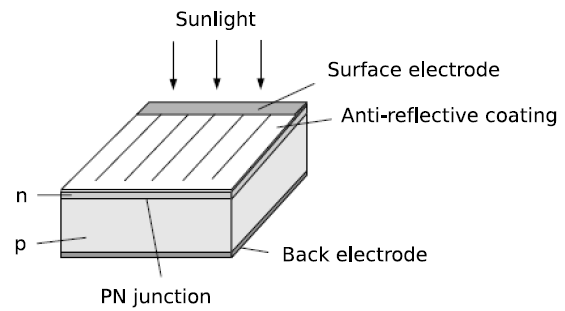
\includegraphics[width=0.5\textwidth]{fig/solarCellStructure.png}
        \caption{The Structure of a Crystalline Silicon Solar Cell.}
        \label{fig:struct}
    \end{figure}
    It is made up of $n/p$ homo-junctions, a 10cm$\times$ 10cm $p$-type silicon plate of thickness $500\mu\rm m$, covered with a heavily doped $n$-type layer with thickness $0.3\mu\rm m$. The metallic bars on the n-type layer serve as one electrode, with a metallic film at the bottom playing the role of another one. In order to reduce the loss of energy due to reflection, an anti-reflective film is often applied to cover the surface exposed to sunlight.
    \subsection{Photovoltatic Effect}
    \paragraph{} When the light enters the $p$-$n$ junction near the solar cell surface, and the energy of the photon ($E=h\nu$) is larger than the energy gap ($E_g$), the photon's energy is absorbed and the electron-hole pair is excited. Minority charge carriers in the $n$- or $p$-area diffuse due to their density gradient. Some of the carriers can diffuse to the region of the $p$-$n$ junction zone, where there is a built-in electric field. Under the electric force, these carriers either move to the $n$-type area (in case of the electron) or move to the $p$-type area (in case of the hole). As a result, the negative charge accumulates in the $n$-type area, and positive charge accumulates in the $p$-type area, and a photoelectric potential difference is generated. The phenomenon described above is known as the \emph{photovoltaic effect}.
    \subsection{Solar Cell Parameters}
    \paragraph{} Because of the photovoltatic effect, the solar cells can generate an electric current $I_{\rm ph}$ from the $n$-type area to the $p$-type area when there is light incident on the solar cell. Meanwhile, in this device there is a forward diode current $I_{\rm D}$ from the $p$-type to the $n$-type area, opposite to $I_{\rm ph}$. In the end, the net current is 
    \begin{equation}
        I=I_{\rm ph}-I_{\rm D}=I_{\rm ph}-I_0\left[\exp\left(\frac{qV_{\rm D}}{nk_{\rm B}T}\right)-1\right],
        \label{eqn:current}
    \end{equation}
    where $V_{\rm D}$ is the junction voltage, $I_0$ is diode inverse saturation current, $I_{\rm ph}$ is the photocurrent determined by the structure and material characteristics of the solar cell. The coefficient $n$ is a theoretical coefficient, with its values ranging from 1 to 2, that characterize the $p$-$n$ junction. In addition, $q$ is the electron's charge, $k_{\rm B}$ is the Boltzmann's constant, and $T$ is the temperature in Kelvin scale. If we neglect the internal series resistance $R_{\rm s}$, the voltage $V_{\rm D}$ is equal to the terminal voltage $V$ and Equation \ref{eqn:current} can be rewritten as $$I=I_{\rm ph}-I_0\left[\exp\left(\frac{qV}{nk_{\rm B}T}\right)-1\right].$$ When the output is short, $i.e.$ $V=0$, the short current circuit is $$I_{\rm sc}=I_{\rm ph},$$ whereas when the output is open, $i.e.$ $I=0$, the open-circuit voltage is $$V_{\rm oc}=\frac{nk_{\rm B}T}{q}\ln\left(\frac{I_{\rm sc}}{I_0}+1\right).$$ When there is a load resistance $R$ (with the value of $R$ ranging from zero to infinity), the corresponding $I$-$V$ characteristics curve is shown in Figure \ref{fig:theory}. If for a certain load resistance $R=R_{\rm m}$, the maximum output power $P_{\rm m}$ is reached, then the value of $P_{\rm m}$ is $$P_{\rm m}=V_{\rm m}I_{\rm m},$$
    \begin{figure}[!ht]
        \centering
        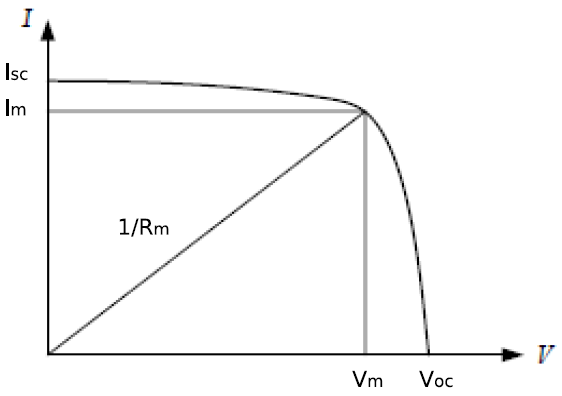
\includegraphics[width=0.5\textwidth]{fig/IVtheory.png}
        \caption{The Theoretical Current-Voltage Characteristics of a Solar Cell.}
        \label{fig:theory}
    \end{figure}
    where $I_{\rm m}$ is the optimal operating current, and $V_{\rm m}$ is the optimal operating voltage. Then, $$FF=\frac{P_{\rm m}}{V_{\rm oc}I_{\rm sc}}=\frac{V_{\rm m}I_{\rm m}}{V_{\rm oc}I_{\rm sc}}.$$ The quantity $FF$ is an important parameter of solar cells called the \emph{fill factor}. The greater the fill factor is, the greater the output power. The fill factor is determined by a number of parameters, such as the incident light intensity, the forbidden bandwidth, the value of the theoretical coeffcient $n$, and the series/parallel resistance.
    \vspace{-5mm}
    \paragraph{}The solar cell energy conversion efficiency $\eta$ is defined as $$\eta=\frac{P_{\rm m}}{P_{\rm in}}\times 100\%,$$ where $P_{\rm in}$ is the total radiant power incident on the solar cell.
    \subsection{Solar Cell Equivalent Circuit}
    \paragraph{}As shown in Figure \ref{fig:equivalentCircuit}, a solar cell can be thought of as composed of a $p$-$n$ junction diode $D$ and a constant current source $I_{\rm ph}$. Along with a series resistance $R_{\rm s}$ due to the electrodes in the solar cell and a parallel resistance $R_{\rm sh}$, all elements form a circuit equivalent to a $p$-$n$ junction leak circuit. For the equivalent circuit one can find the following relationship between the current and the voltage $$I=I_{\rm ph}-I_0\left\{\exp\left[\frac{q(V+R_{\rm s}I)}{nk_{\rm B}T}\right]-1\right\}-\frac{V+R_{\rm s}I}{R_{\rm sh}}.$$ In order to provide a greater output power, the value of $R_{\rm s}$ should be decreased, while $R_{\rm sh}$ should be increased. 
    \begin{figure}[!ht]
        \centering
        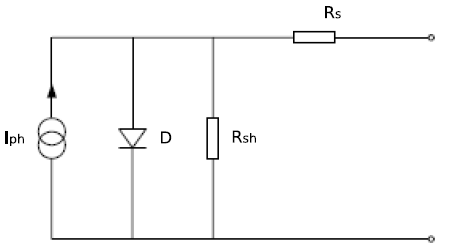
\includegraphics[width=0.5\textwidth]{fig/equivalentCircuit.png}
        \caption{Solar Cell Equivalent Circuit}
        \label{fig:equivalentCircuit}
    \end{figure}
    \section{Apparatus \& Measurement Procedure}
    \subsection{Apparatus}
    \paragraph{}The setup consists of a photovoltaic device (5 W), a 300 W tungsten-halogen lamp serving as a radiation source, two digital multimeters, two adjustable resistors, a solar power meter, a wiring board and a measuring tape. Table \ref{tab:measurement uncertainty} lists the uncertainty of the measurement in this lab. 
    \begin{table}[!ht]
        \centering
        \begin{tabular}{|c|c|}
            \hline
            Quantity&Uncertainty\\\hline
            DC voltage&$\pm(0.5\%+0.01)$[V]\\\hline
            DC current&$\pm(1.5\%+0.1)$[mA]\\\hline
            distance&$\pm 0.1$[cm]\\\hline
            solar power&$\pm 10$[W/m$^2$]\\\hline
        \end{tabular}
        \caption{The Uncertainty of the Measurement}
        \label{tab:measurement uncertainty}
    \end{table}
    \subsection{Measurement Procedure}
    \begin{enumerate}
        \item I(TA) turned on both the light and the fan and waited for more than five minutes, so that the light reached its working intensity.
        \item I, together with my teammates, adjusted the distance of the two lamps from the solar cells to make the open-circuit voltage and the short-circuit current is approximately the same. 
        \item I then measured the length, width of the solar cell and its distance from the lamp with the measuring tape provided. 
        \item Then, I measured the solar power incident on the board with the solar power meter on six different points on the solar cell. 
        \item I measured the open-circuit voltage and short-circuit current for all of the three circuits: series and parallel connection of two solar cells and a single solar cell. 
        \item I then connected the solar cell of these three configurations to a adjustable resistor, and measured the voltage across the resistor and the current through the resistor for 25 different resistance.
        \item Then I change the distance between the lamp and the solar cell, measured the new distance, the new open-circuit voltage and short-circuit current, and 25 more sets of current-voltage relations.
    \end{enumerate}
    \section{Results}
    \subsection{The $I$-$U$ Characteristic Graph}
    \begin{table}[!ht]
        \centering
        \begin{tabular}{|c|c|c|c|c|}
            \hline
            Configurations&$U_{\rm oc}$[V]&Uncertainty[V]&$I_{\rm sc}$[A]&Uncertainty[A]\\\hline
            110.9cm&9.48&0.06&0.0839&0.0014\\\hline
            73.6cm&10.17&0.06&0.162&0.003\\\hline
            series&18.56&0.10&0.0877&0.0014\\\hline
            parallel&9.28&0.06&0.174&0.003\\\hline
        \end{tabular}
        \caption{The Data of $I_{\rm sc}$ and $U_{\rm oc}$ for Different Configurations}
        \label{tab:IVscoc}
    \end{table}
    \begin{figure}[!ht]
        \centering
        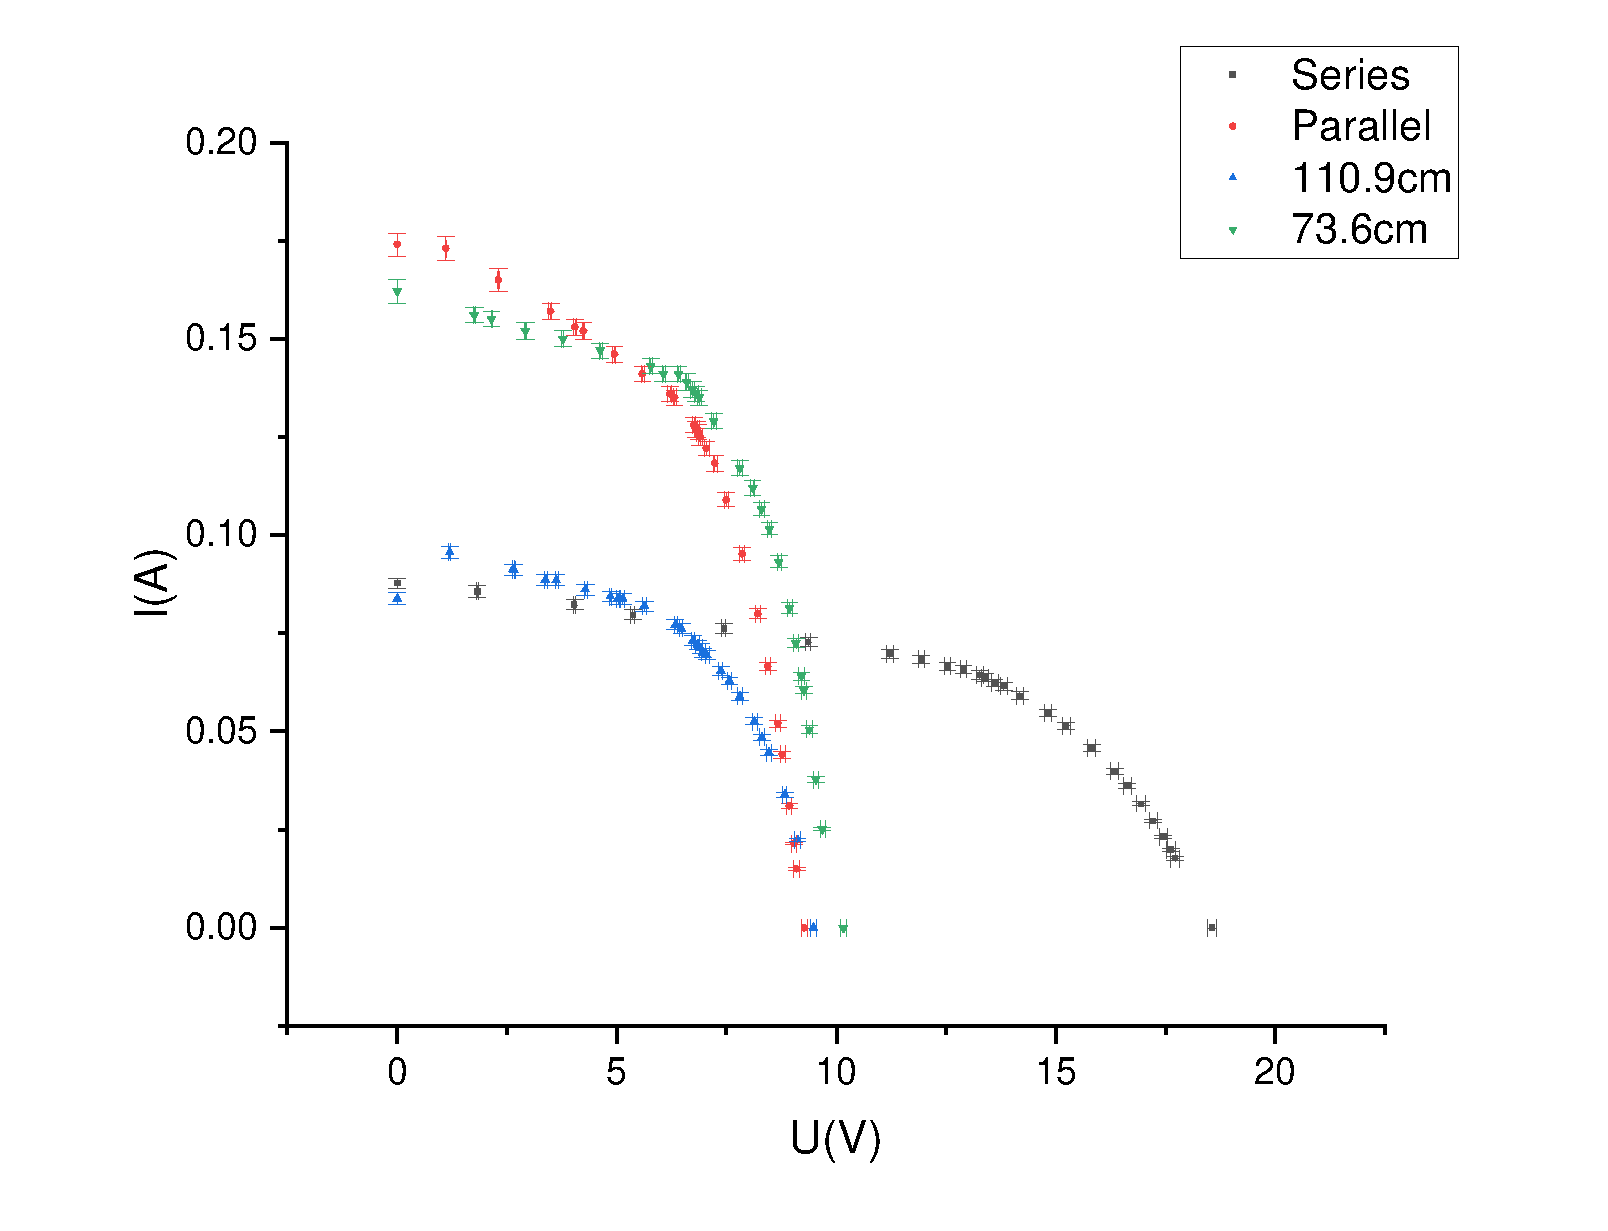
\includegraphics[width=\textwidth]{fig/IvsV.pdf}
        \caption{The $I-U$ Characteristics Curve of the Four Configurations of the Solar Cell}
        \label{fig:IvsV}
    \end{figure}
    \paragraph{} Table \ref{tab:IVsp} and \ref{tab:IVsingle} list a total of 100 sets of data ($I$ vs $U$) in SI unit. The conversion of $I$ from unit [mA] to [A] can be calculated as $I=I'/1000$. For example, when $I'=156.0$[mA], $$I=156.0/1000=0.156[\rm A].$$ Table \ref{tab:IVscoc} lists the short-circuit current and open-circuit voltage for four configurations. And I used these three tables to plot Figure \ref{fig:IvsV}, the $I$-$U$ characteristics of four different (configurations) solar cells.
    \subsection{The $P$-$U$ Relation}
    
    \begin{figure}[!ht]
        \centering
        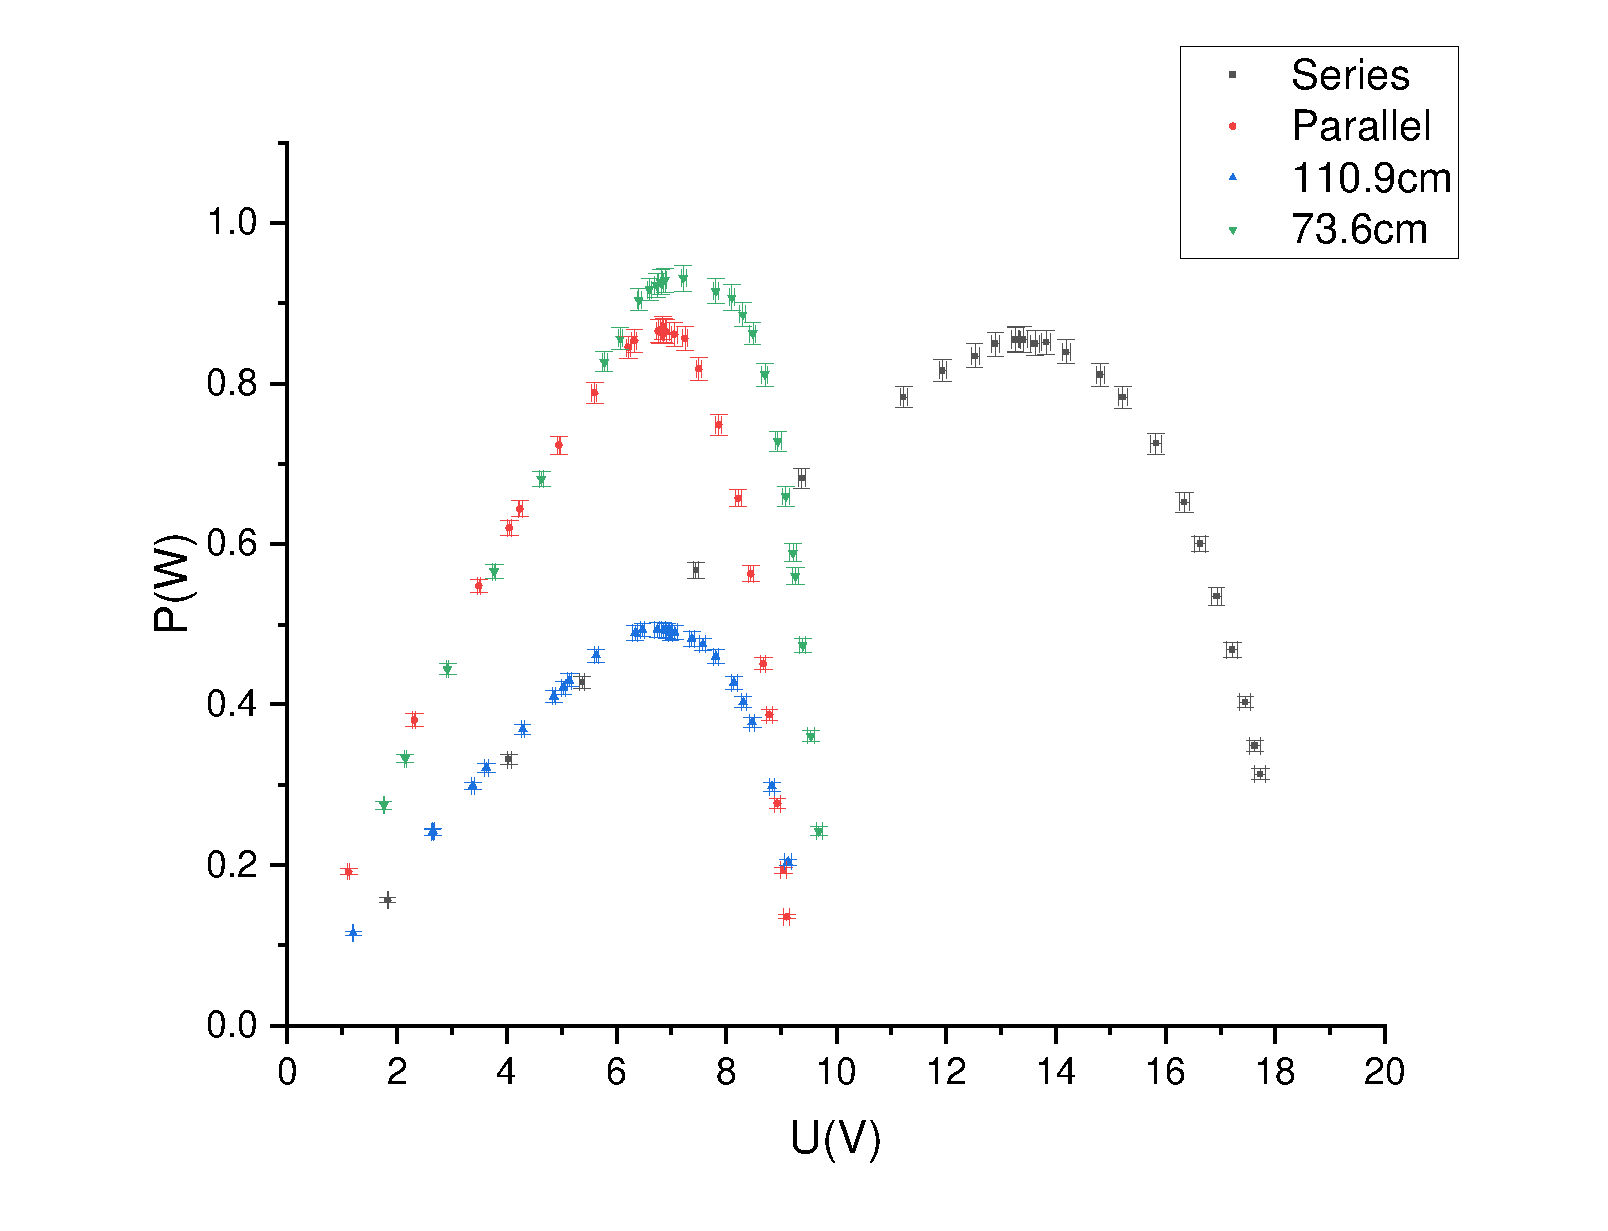
\includegraphics[width=\textwidth]{fig/PvsV.pdf}
        \caption{The relation of $P$ vs. $U$ for Four Configurations of Solar Cells}
        \label{fig:PvsV}
    \end{figure}
    \paragraph{} Table \ref{tab:UPsp} and \ref{tab:PUsingle} list the power-voltage relation of four different configurations of the solar cells. In order to calculated the power, $P=UI$. For example, when $U=1.830$[V], $I=0.0856$[A], $$P=1.830\times 0.0856=0.157[\rm W]\pm 0.003[W].$$ I used these two tables to plot Figure \ref{fig:PvsV}.
    \subsection{The $P$-$R$ Relation}
    
    \begin{figure}[!ht]
        \centering
        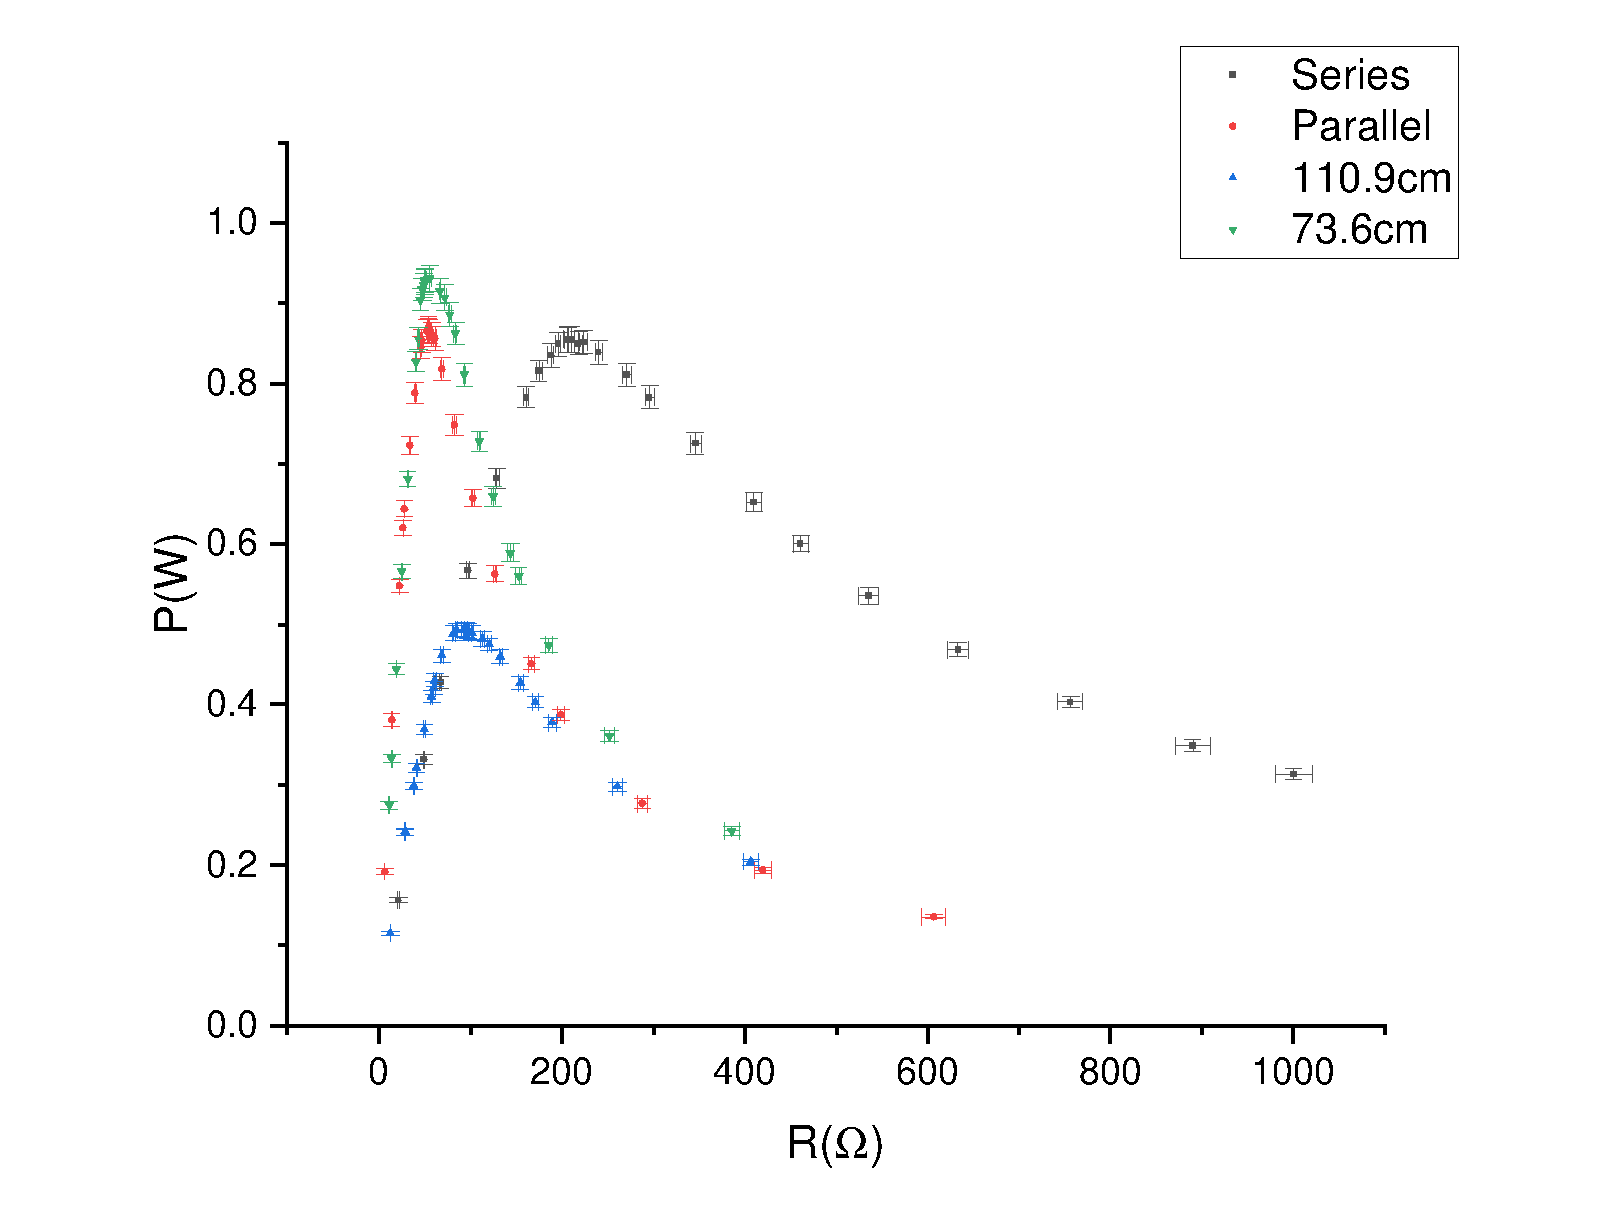
\includegraphics[width=\textwidth]{fig/PvsR.pdf}
        \caption{The relation of $P$ vs. $R$ for Four Configurations of Solar Cells}
        \label{fig:PvsR}
    \end{figure}
    \paragraph{} Table \ref{tab:PvsRsp} and \ref{tab:PRsingle} list the power-resistance relation of four different configurations of solar cells. The (load) resistance is calculated as $R=U/I$. For example, when $U=1.830$[V], $I=0.0856$[A], $$R=\frac{1.830}{0.0856}=21.4[\Omega]\pm 0.4[\Omega].$$
    Then I used these two tables to plot Figure \ref{fig:PvsR}.
    \subsection{The Calculation of Parameters of Each Configuration}
    \paragraph{} We need to obtain eight parameters. $V_{\rm oc}$ and $I_{\rm sc}$ can be obtained directly from Table \ref{tab:IVscoc}. $P_{\rm m}$, $V_{\rm m}$ and $I_{\rm m}$ can be obtained directly from Table \ref{tab:IVsp}, \ref{tab:IVsingle}, \ref{tab:UPsp} and \ref{tab:PUsingle}. $R_{\rm m}$ can be read from Table \ref{tab:PvsRsp} and \ref{tab:PRsingle}. So I will show the calculation of the parameters $FF$ and $\eta$. 
    \vspace{-5mm}
    \paragraph{} The fill factor is given by $$FF=\frac{P_m}{V_{\rm oc}I_{\rm sc}}.$$ For example, in the circuit of distance 110.9[cm], $P_m=0.493$[W], $\V=9.48$[V], $\I=0.0839$[A], and $$FF=\frac{0.493}{9.48\times 0.0839}=0.620\pm 0.016.$$
    \paragraph{} In order to calculate $\eta$, we first need to calculate the total radiation incident on the solar cell. Table \ref{tab:originalpower} shows the original data of the power incident on unit area on the solar cell, and Table \ref{tab:area} shows the length and width of the solar cell. We first calculate the average value of the power on unit area $$\bar{P}=\frac{\sum_{i=1}^6P_i}{6}.$$ When the distance is 110.9[cm], $$\bar{P}=\frac{395+451+389+248+417+268}{6}=360[\rm W/m^2]\pm 80[W/m^2].$$ The area of the solar cell is $S=\text{length}\times \text{width}$. So, $$S=0.255\times 0.206=0.0525[\rm m^2]\pm 0.0003[m^2].$$ And the total power is given as $P_{\rm in}=\bar{P}S$. So, $$P_{\rm in}=360\times 0.0525=19[\rm W]\pm 4[W].$$ Since $\eta=P_{\rm m}/P_{\rm in}\times 100\%$, $$\eta=\frac{0.493}{19}=2.6\%\pm 0.6\%.$$ The same calculation can be applied when the distance is 73.6[cm], and $\eta=2.3\%\pm 0.6\%.$
    \begin{table}[!ht]
        \centering
        \begin{tabular}{|c|c|c|c|c|c|c|}
            \hline
            &1&2&3&4&5&6\\\hline
            $P_{110.9}$[W/m$^2$]&395&451&389&248&417&268\\\hline
            $P_{73.6}$[W/m$^2$]&1160&837&536&783&619&574\\\hline
        \end{tabular}
        \caption{The Power Incident on the Unit Area of a Solar Cell}
        \label{tab:originalpower}
    \end{table}
    \begin{table}[!ht]
        \centering
        \begin{tabular}{|c|c|}
            \hline
            length[cm]&width[cm]\\\hline
            25.5&20.6\\\hline
        \end{tabular}
        \caption{The Length and Width of the Solar Cell}
        \label{tab:area}
    \end{table}
    \begin{table}[!ht]
        \centering
        \begin{tabular}{|c|c|c|c|c|}
            \hline
            &Series&Parallel&110.9[cm]&73.6[cm]\\\hline
            $\V$[V]&$18.56\pm 0.10$&$9.28\pm 0.06$&$9.48\pm 0.06$&$10.17\pm 0.06$\\\hline
            $\I$[A]&$0.0877\pm 0.0014$&$0.174\pm 0.003$&$0.0839\pm 0.0014$&$0.162\pm 0.003$\\\hline
            $P_{\rm m}$[W]&$0.855\pm 0.016$&$0.869\pm 0.015$&$0.493\pm 0.009$&$0.931\pm 0.016$\\\hline
            $V_{\rm m}$[V]&$13.27 \pm 0.08$&$6.84\pm 0.04$&$6.74\pm 0.04$&$7.22\pm 0.05$\\\hline
            $I_{\rm m}$[A]&$0.0644\pm 0.0011$&$0.127\pm 0.002$&$0.0731\pm 0.0012$&$0.129\pm 0.002$\\\hline
            $R_{\rm m}$[$\Omega$]&$206\pm 4$&$53.9\pm 0.9$&$92.2\pm 1.7$&$56.0\pm 1.0$\\\hline
            $FF$&/&/&$0.620\pm 0.016$&$0.565\pm 0.015$\\\hline
            $\eta$&/&/&$2.6\%\pm 0.6\%$&$2.3\%\pm 0.6\%$\\\hline
        \end{tabular}
        \caption{The Parameters of Each Configurations}
        \label{tab:parameter}
    \end{table}
    \section{Discussion}
    \paragraph{} First, we can conclude from Figure \ref{fig:IvsV} that the solar cell is not a linear emf, whose inner resistance should remain a constant, because none of the four $I-U$ characteristics curve is a straight line. However, there is a small problem in this plot. See the blue triangle at $U=0$. It is the short circuit current. It should, in theory, be larger than any other current values. Yet, it lies below some of the triangle points. This is because during the experiment, I first measured the short circuit current and open circuit voltage for 110.9[cm], but when I was measuring the voltage and current for different load resistance, the group next to me moved their lamp to a different configuration, so the short circuit current and the open circuit voltage is not valid any more for this configuration. But besides this false data, the open circuit voltage is larger than any other voltage values and the short circuit current is larger than any other current values. 
    \vspace{-5mm}
    \paragraph{} Second, for the series configuration, while near the maximum power, the power is not monotonic with respect to the resistance any more, $i.e.$, the maximum power is not reached for a certain value of resistance and then declines. In Table \ref{tab:PvsRsp}, we can see that when $R=206, 207, 210[\Omega]$, the power first decreases and then increases, which is a violation of the theory. One possible explanation concerns the uncertainty. By observation, we can see that the uncertainty for both the power and the resistance is not small compared with its value. So the actual maximum value may be closer to the plus side of the uncertainty. 
    \vspace{-5mm}
    \paragraph{} Apart from this, from Figure \ref{fig:PvsV} and \ref{fig:PvsR}, we can conclude that the maximum power transferred to the load reaches the maximum value for a certain value of voltage and resistance. 
    \vspace{-5mm}
    \paragraph{} From Table \ref{tab:parameter}, we can come to many conclusions. First, for maximum power, the voltage of the series configuration is approximately two times of that of the parallel configuration. Also the current of the series is approximately one half of that of the parallel configuration. This is because I adjusted the distance of the two lamps so that the short circuit current and the open circuit voltage is almost the same, so basically it is the parallel or series connection of two identical batteries. For series connection, the open circuit voltage(emf) doubles and the short circuit current remains the same compared to a single solar cell, while for parallel connection, the emf remains the same and the short circuit current doubles. 
    \vspace{-5mm}
    \paragraph{} Second, the efficiency ($\eta$) for both configuration of a single solar cell is small. 2.6\% and 2.3\% are not big numbers, which means that the conversion from the light radiation to electric power is not efficient enough compared to conventional energy sources. 
    \section{Conclusion}
    \paragraph{} In this lab section, I have studied the $I-U$ characteristics curve of the solar cell. In general, the experiment is quite successful, as the theory matches the experiment results quite well. However, there are some minor problems in the experiment listed below and I have given some solutions. 
    \begin{enumerate}
        \item The configuration of the group next to me will affect the result of my own. When they move their lamp, my voltage and current will change. This has caused me some trouble in data analysis. The solution is simple. Make sure the instructor (teaching assistant) tells students that lamps next to each group also affect the experiment result so that the students will ask for permission of the group next to them before they move their lamps. 
        \item Due to the low resolution of the multimeters, the power does not coincide with theory. So getting higher resolution equipment will make the experiment's result more valid and convincing.  
    \end{enumerate}    
    \section{Reference}
    \begin{enumerate}
        \item Qin Tian, Han Xugen, Zheng Huan, Mateusz Krzyzosiak, ``Exercise 3- lab manual [rev. 4.1]''.
    \end{enumerate}
    \renewcommand\thesection{\Alph{section}} 
    \setcounter{section}{0}
    \newpage
    \section{Uncertainty Analysis}
    \subsection{The Uncertainty of $U$ and $I$ for the Original Data}
    \paragraph{} Based on the information given in Table \ref{tab:measurement uncertainty}, the uncertainty of $U$ is $u=U\times 0.5\%+0.01$. For example, when $U=9.12$[V], $$u=9.12\times 0.5\%+0.01=0.06[\rm V].$$
    The uncertainty of $I$ is $u=(I\times 1.5\%+0.1)/1000$. For instance, when $I=25.1$[mA], $$u=\frac{25.1\times 1.5\%+0.1}{1000}=0.0005[\rm A].$$
    The same calculations can be applied to calculate the uncertainty of $U_{\rm oc}$ and $I_{\rm sc}$.
    \subsection{The Uncertainty of $P$ and $R$}
    \paragraph{} The power $P$ is given by $P=UI$, so the uncertainty is 
    \begin{equation*}
        \begin{split}
            u&=\sqrt{\left(\frac{\partial P}{\partial U}u_U\right)^2+\left(\frac{\partial P}{\partial I}u_I\right)^2}\\
            &=\sqrt{I^2u_U^2+U^2u_I^2}
        \end{split}
    \end{equation*} 
    For example, when $U=1.830$[V], $I=0.0856$[A], $u_U=0.019$[V], $u_I=0.0014$[A], the uncertainty is $$u=\sqrt{1.830^2\times 0.0014^2+0.019^2\times 0.0856^2}=0.003[\rm W].$$
    \vspace{-5mm}
    \paragraph{} The (load) resistance is given by $R=U/I$, so the uncertainty is 
    \begin{equation*}
        \begin{split}
            u&=\sqrt{\left(\frac{\partial R}{\partial U}u_U\right)^2+\left(\frac{\partial R}{\partial I}u_I\right)^2}\\
            &=\sqrt{\frac{u_U^2}{I^2}+\frac{U^2u_I^2}{I^4}}\\
            &=\frac{1}{I^2}\sqrt{I^2u_U^2+U^2u_I^2}
        \end{split}
    \end{equation*}
    For example, when $U=1.830$[V], $I=0.0856$[A], $u_U=0.019$[V], $u_I=0.0014$[A], the uncertainty is $$u=\frac{1}{0.0856^2}\times \sqrt{1.830^2\times 0.0014^2+0.019^2\times 0.0856^2}=0.4[\Omega].$$
    \subsection{The Uncertainty of $FF$ and $\eta$}
    \paragraph{} Since $FF={P_m}/{(V_{\rm oc}I_{\rm sc})}$, 
    \begin{equation*}
        \begin{split}
            u&=\sqrt{\left(\frac{\partial FF}{\partial P_m}u_{P_m}\right)^2+\left(\frac{\partial FF}{\partial V_{\rm oc}}u_{V_{\rm oc}}\right)^2+\left(\frac{\partial FF}{\partial I_{\rm sc}}u_{I_{\rm sc}}\right)^2}\\
            &=\sqrt{\frac{u_{P_m}^2}{\V^2\I^2}+\frac{P_m^2u_\V^2}{\V^4\I^2}+\frac{P_m^2u_\I^2}{\I^4\V^2}}\\
            &=\frac{1}{\V^2\I^2}\sqrt{u_{P_m}^2\V^2\I^2+P_m^2u_\V^2\I^2+P_m^2u_\I^2\V^2}.
        \end{split}
    \end{equation*}
    For example, in the series circuit, $P_m=0.493$[W], $\V=9.48$[V], $\I=0.0839$[A], $u_{P_m}=0.009$[W], $u_\V=0.06$[V], $u_\I=0.0014$[A], so the uncertainty is 
    \begin{equation*}
        \begin{split}
            u&=\frac{1}{9.48^2\times 0.0839^2}\sqrt{0.009^2\times 9.48^2\times 0.0839^2+0.493^2\times 0.06^2\times 0.0839^2+0.493^2\times 0.0014^2\times 9.48^2}\\
            &=0.016.
        \end{split}    
    \end{equation*}
    \paragraph{} To calculate the uncertainty of $\eta$, we first consider the uncertainty of the mean value of the six sets of power on unit area. $$u=\sqrt{\Delta_A^2+\Delta_B^2},$$ where $\Delta_B=10[\rm W/m^2]$. $\Delta_A$ is given as $$\Delta_A=s_X\frac{t_{0.95}}{\sqrt{n}}.$$ Since $n=6$ for my measurement, $\frac{t_{0.95}}{\sqrt n}=1$ and $\Delta_A=s_X$. The standard deviation is calculated as $$s_X=\sqrt{\frac{1}{5}\sum_{i=1}^6(P_i-\bar{P})^2}.$$ So when the distance is 110.9[cm], 
    \begin{equation*}
        \begin{split}
            s_X&=\sqrt{\frac{1}{5}((395-360)^2+(451-360)^2+(389-360)^2+(248-360)^2+(417-360)^2+(268-360)^2)}\\
            &=75.9[\rm W/m^2].
        \end{split}
    \end{equation*}
    So, $$u_{\bar{P}}=\sqrt{10^2+75.9^2}=80[\rm W/m^2].$$ Then the uncertainty of the area is given as $$u_S=\sqrt{\left(\frac{\partial S}{\partial l}u_l\right)^2+\left(\frac{\partial S}{\partial w}u_w\right)^2}=u_l\sqrt{l^2+w^2}.$$ Here $u_l=0.001[m]$, $l=0.255$[m], $w=0.206$[m], so the uncertainty is $$u_S=0.001\times\sqrt{0.255^2+0.206^2}=0.0003[\rm m^2].$$ Then the uncertainty of the total power is given as 
    \begin{equation*}
        \begin{split}
            u&=\sqrt{u_{\bar{P}}^2S^2+u_S^2\bar{P}^2}.
        \end{split}
    \end{equation*}
    When $\bar{P}=360[\rm W/m^2]$, $u_{\bar{P}}=80[\rm W/m^2]$, $S=0.05[\rm m^2]$, $u_S=0.0003[\rm m^2]$, we get $$u_P=\sqrt{80^2\times 0.05^2+0.0003^2\times 360^2}=4[\rm W].$$ As for $u_\eta$, 
    \begin{equation*}
        \begin{split}
            u_\eta&=\sqrt{\left(\frac{\partial \eta}{\partial P_{\rm in}}u_{P_{\rm in}}\right)^2+\left(\frac{\partial \eta}{\partial P_{\rm m}}u_{P_{\rm m}}\right)^2}\\
            &=\frac{1}{P_{\rm in}^2}\sqrt{P_{\rm in}^2u_{P_{\rm m}}^2+P_{\rm m}^2u_{P_{\rm in}}^2}
        \end{split}
    \end{equation*}
    Here, $P_{\rm in}=19$[W], $u_{P_{\rm in}}=4$[W], $P_{\rm m}=0.493$[W], $u_{P_{\rm m}}=0.009$[W], and then the uncertainty is 
    \begin{equation*}
        \begin{split}
            u&=\frac{1}{19^2}\times \sqrt{19^2\times 0.009^2+4^2\times 0.493^2}\\
            &=0.006=0.6\%
        \end{split}
    \end{equation*} 
    The same calculation can be applied to the $\eta$ when the distance is 73.6[cm]. $u_\eta=0.6\%$.
    \section{The Data Tables Used to Plot}
    \begin{table}[H]
        \centering
        \begin{tabular}{|c|c|c|c||c|c|c|c|}
            \hline
            \multicolumn{4}{|c||}{series}&\multicolumn{4}{c|}{parallel}\\\hline
            $U$[V]&Uncertainty[V]&$I$[A]&Uncertainty[A]&$U$[V]&Uncertainty[V]&$I$[A]&Uncertainty[A]\\\hline
            1.830&0.019&0.0856&0.0014&1.110&0.016&0.173&0.003\\\hline
            4.04&0.03&0.0822&0.0013&2.31&0.02&0.165&0.003\\\hline
            5.37&0.04&0.0797&0.0013&3.49&0.03&0.157&0.002\\\hline
            7.44&0.05&0.0762&0.0012&4.05&0.03&0.153&0.002\\\hline
            9.37&0.06&0.0728&0.0012&4.24&0.03&0.152&0.002\\\hline
            11.23&0.07&0.0697&0.0011&4.95&0.03&0.146&0.002\\\hline
            11.94&0.07&0.0683&0.0011&5.59&0.04&0.141&0.002\\\hline
            12.53&0.07&0.0666&0.0011&6.21&0.04&0.136&0.002\\\hline
            12.90&0.07&0.0658&0.0011&6.32&0.04&0.135&0.002\\\hline
            13.27&0.08&0.0644&0.0011&6.76&0.04&0.128&0.002\\\hline
            13.28&0.08&0.0643&0.0011&6.80&0.04&0.127&0.002\\\hline
            13.40&0.08&0.0638&0.0011&6.84&0.04&0.127&0.002\\\hline
            13.62&0.08&0.0624&0.0010&6.86&0.04&0.126&0.002\\\hline
            13.82&0.08&0.0616&0.0010&6.91&0.04&0.125&0.002\\\hline
            14.19&0.08&0.0591&0.0010&7.05&0.05&0.1221&0.0019\\\hline
            14.82&0.08&0.0547&0.0009&7.24&0.05&0.1182&0.0019\\\hline
            15.23&0.09&0.0514&0.0009&7.50&0.05&0.1090&0.0017\\\hline
            15.83&0.09&0.0458&0.0008&7.86&0.05&0.0952&0.0015\\\hline
            16.35&0.09&0.0399&0.0007&8.22&0.05&0.0799&0.0013\\\hline
            16.63&0.09&0.0361&0.0006&8.45&0.05&0.0666&0.0011\\\hline
            16.94&0.09&0.0316&0.0006&8.67&0.05&0.0520&0.0009\\\hline
            17.22&0.10&0.0272&0.0005&8.78&0.05&0.0441&0.0008\\\hline
            17.46&0.10&0.0231&0.0004&8.93&0.05&0.0310&0.0006\\\hline
            17.63&0.10&0.0198&0.0004&9.04&0.06&0.0215&0.0004\\\hline
            17.73&0.10&0.0177&0.0004&9.10&0.06&0.0150&0.0003\\\hline
        \end{tabular}
        \caption{The Series and Parallel Solar Cells $I-U$ Relation}
        \label{tab:IVsp}
    \end{table}
    \begin{table}[H]
        \centering
        \begin{tabular}{|c|c|c|c||c|c|c|c|}
            \hline
            \multicolumn{4}{|c||}{110.9[cm]}&\multicolumn{4}{c|}{73.6[cm]}\\\hline
            $U$[V]&Uncertainty[V]&$I$[A]&Uncertainty[A]&$U$[V]&Uncertainty[V]&$I$[A]&Uncertainty[A]\\\hline
            1.200&0.016&0.0956&0.0015&1.760&0.019&0.156&0.002\\\hline
            2.64&0.02&0.0912&0.0015&2.15&0.02&0.155&0.002\\\hline
            2.66&0.02&0.0911&0.0015&2.92&0.02&0.152&0.002\\\hline
            3.38&0.03&0.0886&0.0014&3.77&0.03&0.150&0.002\\\hline
            3.63&0.03&0.0884&0.0014&4.63&0.03&0.147&0.002\\\hline
            4.29&0.03&0.0861&0.0014&5.78&0.04&0.143&0.002\\\hline
            4.86&0.03&0.0844&0.0014&6.07&0.04&0.141&0.002\\\hline
            5.03&0.04&0.0837&0.0014&6.41&0.04&0.141&0.002\\\hline
            5.14&0.04&0.0837&0.0014&6.60&0.04&0.139&0.002\\\hline
            5.63&0.04&0.0819&0.0013&6.73&0.04&0.137&0.002\\\hline
            6.34&0.04&0.0771&0.0013&6.81&0.04&0.136&0.002\\\hline
            6.47&0.04&0.0762&0.0012&6.88&0.04&0.135&0.002\\\hline
            6.74&0.04&0.0731&0.0012&7.22&0.05&0.129&0.002\\\hline
            6.85&0.04&0.0720&0.0012&7.81&0.05&0.1171&0.0019\\\hline
            6.92&0.04&0.0711&0.0012&8.10&0.05&0.1120&0.0018\\\hline
            6.98&0.04&0.0701&0.0012&8.30&0.05&0.1067&0.0017\\\hline
            7.06&0.05&0.0694&0.0011&8.48&0.05&0.1016&0.0016\\\hline
            7.37&0.05&0.0654&0.0011&8.70&0.05&0.0932&0.0015\\\hline
            7.57&0.05&0.0628&0.0010&8.94&0.05&0.0814&0.0013\\\hline
            7.81&0.05&0.0589&0.0010&9.08&0.06&0.0726&0.0012\\\hline
            8.14&0.05&0.0525&0.0009&9.21&0.06&0.0640&0.0011\\\hline
            8.31&0.05&0.0485&0.0008&9.26&0.06&0.0605&0.0010\\\hline
            8.47&0.05&0.0446&0.0008&9.39&0.06&0.0505&0.0009\\\hline
            8.83&0.05&0.0338&0.0006&9.54&0.06&0.0378&0.0007\\\hline
            9.12&0.06&0.0224&0.0004&9.69&0.06&0.0251&0.0005\\\hline
        \end{tabular}
        \caption{The $I-U$ Relation of a Single Solar Cell with Different Distances}
        \label{tab:IVsingle}
    \end{table}
    \begin{table}[H]
        \centering
        \begin{tabular}{|c|c|c|c||c|c|c|c|}
            \hline
            \multicolumn{4}{|c||}{series}&\multicolumn{4}{c|}{parallel}\\\hline
            $U$[V]&Uncertainty[V]&$P$[W]&Uncertainty[W]&$U$[V]&Uncertainty[V]&$P$[W]&Uncertainty[W]\\\hline
            1.830&0.019&0.157&0.003&1.110&0.016&0.192&0.004\\\hline
            4.04&0.03&0.332&0.006&2.31&0.02&0.381&0.008\\\hline
            5.37&0.04&0.428&0.008&3.49&0.03&0.548&0.008\\\hline
            7.44&0.05&0.567&0.010&4.05&0.03&0.620&0.009\\\hline
            9.37&0.06&0.682&0.012&4.24&0.03&0.644&0.010\\\hline
            11.23&0.07&0.783&0.013&4.95&0.03&0.723&0.011\\\hline
            11.94&0.07&0.816&0.014&5.59&0.04&0.788&0.013\\\hline
            12.53&0.07&0.834&0.015&6.21&0.04&0.845&0.014\\\hline
            12.90&0.07&0.849&0.015&6.32&0.04&0.853&0.014\\\hline
            13.27&0.08&0.855&0.015&6.76&0.04&0.865&0.014\\\hline
            13.28&0.08&0.854&0.015&6.80&0.04&0.864&0.015\\\hline
            13.40&0.08&0.855&0.016&6.84&0.04&0.869&0.015\\\hline
            13.62&0.08&0.850&0.015&6.86&0.04&0.866&0.015\\\hline
            13.82&0.08&0.851&0.015&6.91&0.04&0.864&0.015\\\hline
            14.19&0.08&0.839&0.015&7.05&0.05&0.861&0.015\\\hline
            14.82&0.08&0.811&0.014&7.24&0.05&0.856&0.015\\\hline
            15.23&0.09&0.783&0.014&7.50&0.05&0.818&0.014\\\hline
            15.83&0.09&0.725&0.013&7.86&0.05&0.748&0.013\\\hline
            16.35&0.09&0.652&0.012&8.22&0.05&0.657&0.011\\\hline
            16.63&0.09&0.600&0.010&8.45&0.05&0.563&0.010\\\hline
            16.94&0.09&0.535&0.011&8.67&0.05&0.451&0.008\\\hline
            17.22&0.10&0.468&0.009&8.78&0.05&0.387&0.007\\\hline
            17.46&0.10&0.403&0.007&8.93&0.05&0.277&0.006\\\hline
            17.63&0.10&0.349&0.007&9.04&0.06&0.194&0.004\\\hline
            17.73&0.10&0.314&0.007&9.10&0.06&0.136&0.003\\\hline
        \end{tabular}
        \caption{The Series and Parallel Solar Cells $P-U$ Relation}
        \label{tab:UPsp}
    \end{table}
    \begin{table}[H]
        \centering
        \begin{tabular}{|c|c|c|c||c|c|c|c|}
            \hline
            \multicolumn{4}{|c||}{110.9[cm]}&\multicolumn{4}{c|}{73.6[cm]}\\\hline
            $U$[V]&Uncertainty[V]&$P$[W]&Uncertainty[W]&$U$[V]&Uncertainty[V]&$P$[W]&Uncertainty[W]\\\hline
            1.200&0.016&0.115&0.002&1.760&0.019&0.275&0.005\\\hline
            2.64&0.02&0.241&0.004&2.15&0.02&0.333&0.005\\\hline
            2.66&0.02&0.242&0.004&2.92&0.02&0.444&0.007\\\hline
            3.38&0.03&0.299&0.005&3.77&0.03&0.566&0.009\\\hline
            3.63&0.03&0.321&0.006&4.63&0.03&0.681&0.010\\\hline
            4.29&0.03&0.369&0.007&5.78&0.04&0.827&0.013\\\hline
            4.86&0.03&0.410&0.007&6.07&0.04&0.856&0.013\\\hline
            5.03&0.04&0.421&0.008&6.41&0.04&0.904&0.014\\\hline
            5.14&0.04&0.430&0.008&6.60&0.04&0.917&0.014\\\hline
            5.63&0.04&0.461&0.008&6.73&0.04&0.922&0.015\\\hline
            6.34&0.04&0.489&0.009&6.81&0.04&0.926&0.015\\\hline
            6.47&0.04&0.493&0.008&6.88&0.04&0.929&0.015\\\hline
            6.74&0.04&0.493&0.009&7.22&0.05&0.931&0.016\\\hline
            6.85&0.04&0.493&0.009&7.81&0.05&0.915&0.016\\\hline
            6.92&0.04&0.492&0.009&8.10&0.05&0.907&0.016\\\hline
            6.98&0.04&0.489&0.009&8.30&0.05&0.886&0.015\\\hline
            7.06&0.05&0.490&0.009&8.48&0.05&0.862&0.014\\\hline
            7.37&0.05&0.482&0.009&8.70&0.05&0.811&0.014\\\hline
            7.57&0.05&0.475&0.008&8.94&0.05&0.728&0.012\\\hline
            7.81&0.05&0.460&0.008&9.08&0.06&0.659&0.012\\\hline
            8.14&0.05&0.427&0.008&9.21&0.06&0.589&0.011\\\hline
            8.31&0.05&0.403&0.007&9.26&0.06&0.560&0.010\\\hline
            8.47&0.05&0.378&0.007&9.39&0.06&0.474&0.009\\\hline
            8.83&0.05&0.298&0.006&9.54&0.06&0.361&0.007\\\hline
            9.12&0.06&0.204&0.004&9.69&0.06&0.243&0.005\\\hline
        \end{tabular}
        \caption{The $P-U$ Relation of a Single Solar Cell with Different Distances}
        \label{tab:PUsingle}
    \end{table}
    \begin{table}[H]
        \centering
        \begin{tabular}{|c|c|c|c||c|c|c|c|}
            \hline
            \multicolumn{4}{|c||}{series}&\multicolumn{4}{c|}{parallel}\\\hline
            $R$[$\Omega$]&Uncertainty[$\Omega$]&$P$[W]&Uncertainty[W]&$R$[$\Omega$]&Uncertainty[$\Omega$]&$P$[W]&Uncertainty[W]\\\hline
            21.4&0.4&0.157&0.003&6.42&0.13&0.192&0.004\\\hline
            49.1&0.9&0.332&0.006&14.0&0.3&0.381&0.008\\\hline
            67.4&1.3&0.428&0.008&22.2&0.3&0.548&0.008\\\hline
            97.6&1.7&0.567&0.010&26.5&0.4&0.620&0.009\\\hline
            129&2&0.682&0.012&27.9&0.4&0.644&0.010\\\hline
            161&3&0.783&0.013&33.9&0.5&0.723&0.011\\\hline
            175&3&0.816&0.014&39.6&0.7&0.788&0.013\\\hline
            188&3&0.834&0.015&45.7&0.8&0.845&0.014\\\hline
            196&3&0.849&0.015&46.8&0.8&0.853&0.014\\\hline
            206&4&0.855&0.015&52.8&0.9&0.865&0.014\\\hline
            207&4&0.854&0.015&53.5&0.9&0.864&0.015\\\hline
            210&4&0.855&0.016&53.9&0.9&0.869&0.015\\\hline
            218&4&0.850&0.015&54.4&0.9&0.866&0.015\\\hline
            224&4&0.851&0.015&55.3&1.0&0.864&0.015\\\hline
            240&4&0.839&0.015&57.7&1.0&0.861&0.015\\\hline
            271&5&0.811&0.014&61.3&1.1&0.856&0.015\\\hline
            296&5&0.783&0.014&68.8&1.2&0.818&0.014\\\hline
            346&6&0.725&0.013&82.6&1.4&0.748&0.013\\\hline
            410&8&0.652&0.012&102.9&1.7&0.657&0.011\\\hline
            461&8&0.600&0.010&127&2&0.563&0.010\\\hline
            536&11&0.535&0.011&167&3&0.451&0.008\\\hline
            633&12&0.468&0.009&199&4&0.387&0.007\\\hline
            756&13&0.403&0.007&288&6&0.277&0.006\\\hline
            890&18&0.349&0.007&420&9&0.194&0.004\\\hline
            1000&20&0.314&0.007&607&13&0.136&0.003\\\hline
        \end{tabular}
        \caption{The Series and Parallel Solar Cells $P-R$ Relation}
        \label{tab:PvsRsp}
    \end{table}
    \begin{table}[H]
        \centering
        \begin{tabular}{|c|c|c|c||c|c|c|c|}
            \hline
            \multicolumn{4}{|c||}{110.9[cm]}&\multicolumn{4}{c|}{73.6[cm]}\\\hline
            $R$[$\Omega$]&Uncertainty[$\Omega$]&$P$[W]&Uncertainty[W]&$R$[$\Omega$]&Uncertainty[$\Omega$]&$P$[W]&Uncertainty[W]\\\hline
            12.6&0.2&0.115&0.002&11.3&0.2&0.275&0.005\\\hline
            28.9&0.5&0.241&0.004&13.9&0.2&0.333&0.005\\\hline
            29.2&0.5&0.242&0.004&19.2&0.3&0.444&0.007\\\hline
            38.1&0.6&0.299&0.005&25.1&0.4&0.566&0.009\\\hline
            41.1&0.8&0.321&0.006&31.5&0.5&0.681&0.010\\\hline
            49.8&0.9&0.369&0.007&40.4&0.6&0.827&0.013\\\hline
            57.6&1.0&0.410&0.007&43.0&0.7&0.856&0.013\\\hline
            60.1&1.1&0.421&0.008&45.5&0.7&0.904&0.014\\\hline
            61.4&1.1&0.430&0.008&47.5&0.7&0.917&0.014\\\hline
            68.7&1.2&0.461&0.008&49.1&0.8&0.922&0.015\\\hline
            82.2&1.5&0.489&0.009&50.1&0.8&0.926&0.015\\\hline
            84.9&1.4&0.493&0.008&51.0&0.8&0.929&0.015\\\hline
            92.2&1.7&0.493&0.009&56.0&1.0&0.931&0.016\\\hline
            95.1&1.7&0.493&0.009&66.7&1.2&0.915&0.016\\\hline
            97.3&1.8&0.492&0.009&72.3&1.3&0.907&0.016\\\hline
            99.6&1.8&0.489&0.009&77.8&1.3&0.886&0.015\\\hline
            101.7&1.9&0.490&0.009&83.5&1.4&0.862&0.014\\\hline
            113&2&0.482&0.009&93.3&1.6&0.811&0.014\\\hline
            121&2&0.475&0.008&109.8&1.8&0.728&0.012\\\hline
            133&2&0.460&0.008&125&2&0.659&0.012\\\hline
            155&3&0.427&0.008&144&3&0.589&0.011\\\hline
            171&3&0.403&0.007&153&3&0.560&0.010\\\hline
            190&4&0.378&0.007&186&4&0.474&0.009\\\hline
            261&5&0.298&0.006&252&5&0.361&0.007\\\hline
            407&8&0.204&0.004&386&8&0.243&0.005\\\hline
        \end{tabular}
        \caption{The $P-R$ Relation of a Single Solar Cell with Different Distances}
        \label{tab:PRsingle}
    \end{table}
    \section{Data Sheet}
    \paragraph{} The original data sheet is attached to this report.
\end{document}
